%
% teil3.tex -- Beispiel-File für Teil 7
%
% (c) 2020 Prof Dr Andreas Müller, Hochschule Rapperswil
%
% !TEX root = ../../buch.tex
% !TEX encoding = UTF-8
%
\section{Spezialfall reelle Zahlen
\label{moebius:section:teil7}}
\kopfrechts{Spezialfall reelle Zahlen}

\subsection{Möbius-Transformationen auf der reellen Achse}
Betrachtet man Möbius-Transformationen der Form
\[
f(z) = \frac{az + b}{cz + d}
\]
und schränkt die Variable auf reelle Zahlen ein, also \( z = x \in \mathbb{R} \),
so erhält man die reelle Funktion
\[
f(x) = \frac{ax + b}{cx + d}.
\]
Dabei werden reelle Zahlen wieder auf reelle Zahlen abgebildet (sofern \(cx + d \neq 0\)).
\medskip
\\
\subsection{Interpretation der Parameter}
Die Parameter \(a, b, c, d\) bestimmen die Art der Transformation:
\begin{itemize}
	\item \(a\): bewirkt eine Skalierung (Streckung im reellen Fall)
	\item \(b\): entspricht einer Verschiebung (Translation)
	\item \(c\): erzeugt eine nichtlineare Verzerrung (insbesondere Inversionseffekte)
	\item \(d\): beeinflusst die Lage der Polstelle (Singularität)
\end{itemize}
\medskip
Eine wichtige Eigenschaft ist, dass alle Punkte bleiben auf der reellen Achse, das heisst:
\[
f : \mathbb{R} \to \mathbb{R} \cup \{\infty\}.
\]
Die Transformation ist also eine Abbildung der erweiterten reellen Zahlengeraden.
\medskip
\\
\subsection{Geometrische Interpretation}
Während Möbius-Transformationen in der komplexen Ebene Kreise und Geraden
ineinander überführen, reduziert sich dies im reellen Fall auf Transformationen der Geraden.
Es entstehen keine Kreise in der Ebene, da nur eine Dimension betrachtet wird.
Ein Kreis in der Ebene hat die Form
\[
x^2 + y^2 = r^2,
\]
benötigt also zwei Dimensionen. Für reelle Zahlen gilt jedoch \(y = 0\),
sodass alle Punkte auf der \(x\)-Achse liegen.
Möbius-Transformationen auf der reellen Achse sind gebrochen-rationale Funktionen der Form
\index{gebrochen-rational}%
\[
f(x) = \frac{ax + b}{cx + d}, \quad ad - bc \neq 0,
\]
die die erweiterte reelle Zahlengerade \(\mathbb{R} \cup \{\infty\}\) bijektiv auf sich selbst abbilden.
Diese Transformationen bilden die Grundlage der projektiven Geometrie auf der reellen Geraden.
\begin{figure}
	\centering
	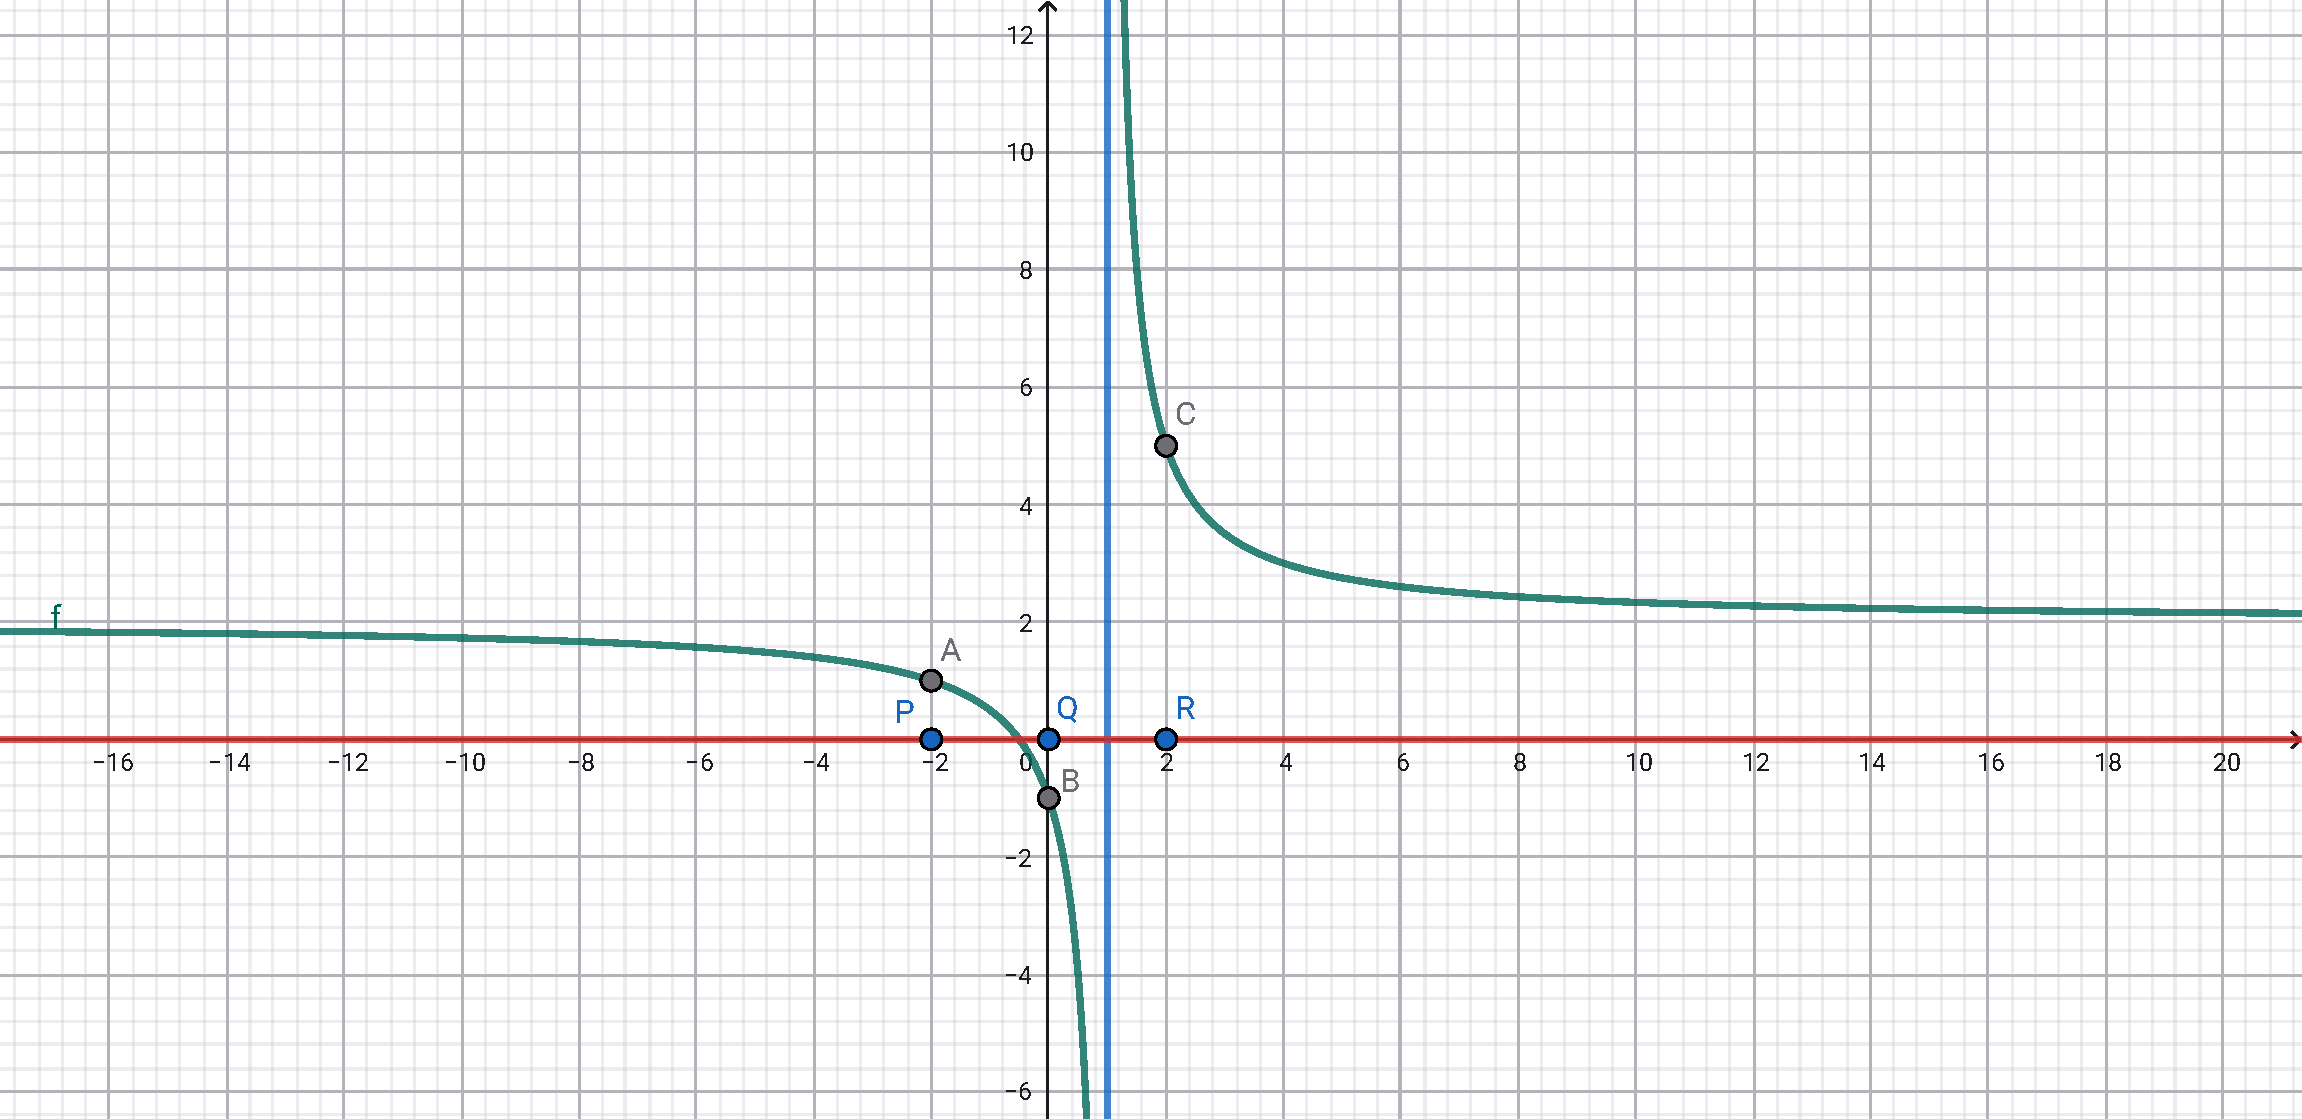
\includegraphics[width=1\textwidth]{papers/moebius/bild10.pdf}
	\caption{Spezialfall reelle Zahlen (erstellt mit GeoGebra)}
\end{figure}
Die Eingabewerte \(x \in \mathbb{R}\) liegen auf der x-Achse, während die Funktionswerte durch eine gebrochen-rationale Funktion beschrieben werden. 
Die Funktion besitzt eine Polstelle bei \(x = -\frac{d}{c}\), an der sie gegen \(\infty\) divergiert (falls \(c \neq 0\)). 
\index{Polstelle}%
Für grosse Beträge von \(x\) nähert sich der Funktionsgraph der horizontalen Asymptote \(y = \frac{a}{c}\).
